
\Large


\chapter{Orthogonal Projections}

A projection is a linear operator \( P \) satisfying \( P^2 = P \). One can think of \( P \) as a transformation that \textbf{fixes every vector in its column space}—that is, if \( \mathbf{v} \in \operatorname{Col}(P) \), then \( P\mathbf{v} = \mathbf{v} \). 

Given any vector \( \mathbf{x} \), we can decompose it as  
\[
\mathbf{x} = P\mathbf{x} + (\mathbf{x} - P\mathbf{x}),
\]  
where:
\begin{itemize}
\item \( P\mathbf{x} \) is the \textbf{projected part}, lying in \( \operatorname{Col}(P) \);
    \item \( \mathbf{x} - P\mathbf{x} \) is the \textbf{residual} (or error), which lies in the \textbf{null space} \( \operatorname{Nul}(P) \), because 
    \[
    P(\mathbf{x} - P\mathbf{x}) = P\mathbf{x} - P^2\mathbf{x} = P\mathbf{x} - P\mathbf{x} = \mathbf{0}.
    \]
\end{itemize}
Thus, the entire space splits as a \textbf{direct sum}:  
\[
\mathbb{R}^n = \operatorname{Col}(P) \oplus \operatorname{Nul}(P).
\]  
Every vector can be written uniquely as a sum of a vector in the column space and a vector in the null space.

An \textbf{orthogonal projection} can be described in two seemingly different ways:

\begin{enumerate}
    \item \textbf{Geometrically}: a projection \( P \) is orthogonal if its column space and null space are perpendicular, i.e.,  
    \[
    \operatorname{Col}(P) \perp \operatorname{Nul}(P).
    \]

    \item \textbf{Algebraically}: a projection \( P \) is orthogonal if it is symmetric, i.e.,  
    \[
    P^\top = P.
    \]
\end{enumerate}


The purpose of this note is to \textbf{prove the equivalence of these two definitions}. That is, for any matrix \( P \) satisfying \( P^2 = P \), we will show:
\[
\operatorname{Col}(P) \perp \operatorname{Nul}(P) \quad \Longleftrightarrow \quad P^\top = P.
\]






\newpage

\begin{theorem}[The Orthogonal Projection Theorem]
Let \( P \) be a linear operator on \( \mathbb{R}^n \) such that \( P^2 = P \) (i.e., \( P \) is a projection).  
Then the following are equivalent:
\begin{enumerate}
    \item \( P \) is an \textbf{orthogonal projection}, meaning \( \operatorname{Col}(P) \perp \operatorname{Nul}(P) \);
    \item \( P \) is \textbf{symmetric}, i.e., \( P^\top = P \).
\end{enumerate}
In other words, for a projection, symmetry is equivalent to orthogonality of the column and null spaces.
\end{theorem}

\begin{proof}
We prove both directions.

\medskip
\noindent\textbf{(1) Symmetry \( \implies \) Orthogonality.}  
Assume \( P^2 = P \) and \( P^\top = P \).  
By the Fundamental Theorem of Linear Algebra,
\[
\operatorname{Col}(P)^\perp = \operatorname{Nul}(P^\top).
\]
Since \( P \) is symmetric, \( P^\top = P \), so \( \operatorname{Nul}(P^\top) = \operatorname{Nul}(P) \). Hence,
\[
\operatorname{Col}(P)^\perp = \operatorname{Nul}(P),
\]
which means \( \operatorname{Col}(P) \perp \operatorname{Nul}(P) \). Thus, \( P \) is an orthogonal projection.

\medskip
\noindent\textbf{(2) Orthogonality \( \implies \) Symmetry.}  
Assume \( P^2 = P \) and \( \operatorname{Col}(P) \perp \operatorname{Nul}(P) \).  
Then \( \operatorname{Nul}(P) = \operatorname{Col}(P)^\perp \). Again by the Fundamental Theorem,
\[
\operatorname{Col}(P)^\perp = \operatorname{Nul}(P^\top),
\]
so we obtain
\[
\operatorname{Nul}(P) = \operatorname{Nul}(P^\top).
\]

To show \( P = P^\top \), it suffices to verify that for all vectors \( \mathbf{x}, \mathbf{y} \in \mathbb{R}^n \),
\[
\mathbf{x}^\top P \mathbf{y} = \mathbf{x}^\top P^\top \mathbf{y}.
\]

Because \( P \) is an orthogonal projection, every vector decomposes orthogonally as
\[
\mathbf{z} = P\mathbf{z} + (\mathbf{z} - P\mathbf{z}), \quad \text{with } P\mathbf{z} \in \operatorname{Col}(P),\; \mathbf{z} - P\mathbf{z} \in \operatorname{Nul}(P).
\]

Now consider arbitrary \( \mathbf{x}, \mathbf{y} \). Since \( \mathbf{x} - P\mathbf{x} \in \operatorname{Nul}(P) \) and \( P\mathbf{y} \in \operatorname{Col}(P) \), orthogonality gives
\[
(\mathbf{x} - P\mathbf{x})^\top P\mathbf{y} = 0
\quad\Longrightarrow\quad
\mathbf{x}^\top P\mathbf{y} = (P\mathbf{x})^\top P\mathbf{y}. \tag{*}
\]

Similarly, \( P\mathbf{x} \in \operatorname{Col}(P) \) and \( \mathbf{y} - P\mathbf{y} \in \operatorname{Nul}(P) \) are orthogonal, so
\[
(P\mathbf{x})^\top (\mathbf{y} - P\mathbf{y}) = 0
\quad\Longrightarrow\quad
(P\mathbf{x})^\top \mathbf{y} = (P\mathbf{x})^\top P\mathbf{y}. \tag{**}
\]

From (*) and (**), we conclude
\[
\mathbf{x}^\top P\mathbf{y} = (P\mathbf{x})^\top \mathbf{y} = \mathbf{x}^\top P^\top \mathbf{y}.
\]
Since this holds for all \( \mathbf{x}, \mathbf{y} \), it follows that \( P = P^\top \).

\medskip
Thus, the two conditions are equivalent.
\end{proof}

\section{Finding particular projection matrices}



\Large

Now that we understand what an orthogonal projection is, we would like to be able to construct explicit matrices which project onto a given subspace. Let us begin with the one dimensional case.

\section*{Goal}

Let $ \mathbf{u}_1 \in \mathbb{R}^n $ be a unit vector (i.e., $ \|\mathbf{u}_1\| = 1 $).  
We want to find the matrix $ P $ that orthogonally projects any vector $ \mathbf{x} \in \mathbb{R}^n $ onto the line spanned by $ \mathbf{u}_1 $.

\section*{Geometric Definition of Orthogonal Projection}

The orthogonal projection $ \hat{\mathbf{x}} = P\mathbf{x} $ must satisfy:
\begin{enumerate}
    \item $ \hat{\mathbf{x}} $ lies on the line: $ \hat{\mathbf{x}} = c \mathbf{u}_1 $ for some scalar $ c $,
    \item The error $ \mathbf{x} - \hat{\mathbf{x}} $ is perpendicular to the line: $ (\mathbf{x} - \hat{\mathbf{x}})^\top \mathbf{u}_1 = 0 $.
\end{enumerate}

\section*{Deriving the Projection Formula}

From condition (2):
\[
(\mathbf{x} - c \mathbf{u}_1)^\top \mathbf{u}_1 = 0
\quad \Rightarrow \quad
\mathbf{x}^\top \mathbf{u}_1 - c \, \mathbf{u}_1^\top \mathbf{u}_1 = 0.
\]
Since $ \mathbf{u}_1 $ is a unit vector, $ \mathbf{u}_1^\top \mathbf{u}_1 = 1 $, so
\[
c = \mathbf{u}_1^\top \mathbf{x}.
\]
Thus, the projection is
\[
\hat{\mathbf{x}} = (\mathbf{u}_1^\top \mathbf{x}) \, \mathbf{u}_1.
\]

\section*{Expressing as a Matrix Multiplication}

We now seek a matrix $ P $ such that $ \hat{\mathbf{x}} = P\mathbf{x} $ for all $ \mathbf{x} $.  
Rewrite the expression using the fact that $(\mathbf{u}_1^\top \mathbf{x})$ is a scalar together with the associativity of matrix multiplication:
\[
\hat{\mathbf{x}} = (\mathbf{u}_1^\top \mathbf{x}) \, \mathbf{u}_1
= \mathbf{u}_1 (\mathbf{u}_1^\top \mathbf{x})
= (\mathbf{u}_1 \mathbf{u}_1^\top) \mathbf{x}.
\]
Since this holds for every $ \mathbf{x} $, we identify
\[
P = \mathbf{u}_1 \mathbf{u}_1^\top.
\]

\section*{Verifying Projection Properties}

\begin{itemize}
\item \textbf{Idempotent}: 
    \[
    P^2 = (\mathbf{u}_1 \mathbf{u}_1^\top)(\mathbf{u}_1 \mathbf{u}_1^\top)
    = \mathbf{u}_1 (\mathbf{u}_1^\top \mathbf{u}_1) \mathbf{u}_1^\top
    = \mathbf{u}_1 (1) \mathbf{u}_1^\top = P.
    \]

    \item \textbf{Symmetric}:
    \[
    P^\top = (\mathbf{u}_1 \mathbf{u}_1^\top)^\top = \mathbf{u}_1 \mathbf{u}_1^\top = P.
    \]
Thus, $ P $ is an orthogonal projection matrix.
\end{itemize}

\section*{Geometric Interpretation}

The matrix $ \mathbf{u}_1 \mathbf{u}_1^\top $ is the \textbf{outer product} of $ \mathbf{u}_1 $ with itself.  
- The inner product $ \mathbf{u}_1^\top \mathbf{x} $ gives the scalar coordinate along $ \mathbf{u}_1 $,
- The outer product $ \mathbf{u}_1 \mathbf{u}_1^\top $ converts this into a linear transformation that projects any vector onto the line.

\section*{Example: 2D Projection}

Let $ \mathbf{u}_1 = \begin{bmatrix} \cos \theta \\ \sin \theta \end{bmatrix} $. Then
\[
P = \mathbf{u}_1 \mathbf{u}_1^\top =
\begin{bmatrix}
\cos^2 \theta & \cos \theta \sin \theta \\
\cos \theta \sin \theta & \sin^2 \theta
\end{bmatrix},
\]
This is the standard orthogonal projection matrix onto a line at angle $ \theta $.
To see this let \( L \) be the line through the origin in \( \mathbb{R}^2 \) that makes an angle \( \theta \) with the positive \( x \)-axis.  



\begin{center}
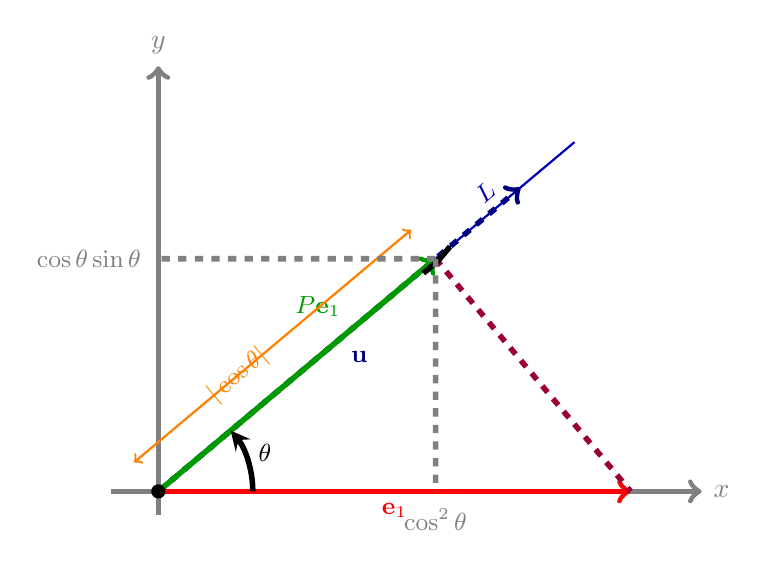
\begin{tikzpicture}[scale=6, line width=2pt]
    % Define angle in degrees for calculations
    \def\AngleValue{40}

    % Compute trig values
    \pgfmathsetmacro{\cost}{cos(\AngleValue)}
    \pgfmathsetmacro{\sint}{sin(\AngleValue)}
    \pgfmathsetmacro{\xP}{\cost*\cost}
    \pgfmathsetmacro{\yP}{\cost*\sint}

    % Points
    \coordinate (O) at (0,0);
    \coordinate (A) at (1,0);
    \coordinate (P) at (\xP, \yP);
    \coordinate (U) at (\cost, \sint);

    % Axes
    \draw[->, gray] (-0.1,0) -- (1.15,0) node[right] {$x$};
    \draw[->, gray] (0,-0.05) -- (0,0.9) node[above] {$y$};

    % Line L
    \draw[thick, blue!70!black] (O) -- ({1.15*\cost}, {1.15*\sint}) node[pos=0.85, above left, sloped, font=\small] {$L$};

    % Unit vector
    \draw[dashed, ->, blue!50!black] (O) -- (U) node[midway, below right, font=\small] {$\mathbf{u}$};

    % e1
    \draw[->, red] (O) -- (A) node[midway, below, font=\small] {$\mathbf{e}_1$};

    % Projection
    \draw[->, green!60!black] (O) -- (P) node[pos=0.7, above left, font=\small] {$P\mathbf{e}_1$};

    % Residual
    \draw[dashed, purple!80!black] (P) -- (A);

    % Right angle
    \draw[shift={(P)}] ({-0.04*\sint}, {-0.04*\cost}) -- ({-0.04*\sint + 0.04*\cost}, {-0.04*\cost + 0.04*\sint}) -- ({0.04*\cost}, {0.04*\sint});

    % Length label (offset from OP line)
    \pgfmathsetmacro{\offset}{0.08} % Small offset for the label
    \coordinate (O_off) at ({-\offset*\sint}, {\offset*\cost});
    \coordinate (P_off) at ({\xP - \offset*\sint}, {\yP + \offset*\cost});
    \draw[<->, orange, thick] (O_off) -- (P_off) node[midway, left, font=\small, sloped] {$\vert\cos\theta\vert$};

    % Coordinate drops
    \draw[dashed, gray] (P) -- (\xP, 0) node[below, font=\small, yshift=-2pt] {$\cos^2\theta$};
    \draw[dashed, gray] (P) -- (0, \yP) node[left, font=\small, xshift=-2pt] {$\cos\theta\sin\theta$};

    % Angle arc
    \draw[->, >=stealth] (0.2,0) arc (0:\AngleValue:0.2);
    \node[font=\small] at ({0.24*cos(\AngleValue/2)}, {0.24*sin(\AngleValue/2)}) {$\theta$};

    % Origin
    \fill (O) circle (0.015);
\end{tikzpicture}
\end{center}

 
We consider the \textbf{orthogonal projection} of the vector \( \mathbf{e}_1 = \begin{bmatrix} 1 \\ 0 \end{bmatrix} \) onto \( L \).  
We will show geometrically that the projected point has coordinates
\[
\bigl( \cos^2\theta,\; \cos\theta \sin\theta \bigr).
\]

\subsection*{Step 1: The length of the projection is \( \cos\theta \)}

The direction of the line \( L \) is given by the \textbf{unit vector}
\[
\mathbf{u} = \begin{bmatrix} \cos\theta \\ \sin\theta \end{bmatrix}.
\]
The orthogonal projection of any vector \( \mathbf{x} \) onto \( L \) lies along \( \mathbf{u} \), at a distance equal to the scalar component of \( \mathbf{x} \) in the direction of \( \mathbf{u} \).

For \( \mathbf{x} = \mathbf{e}_1 = (1, 0) \), this scalar component is the dot product:
\[
\mathbf{u}^\top \mathbf{e}_1 = \cos\theta \cdot 1 + \sin\theta \cdot 0 = \cos\theta.
\]
Thus, the projected point \( P \) lies on \( L \), at a distance \( \cos\theta \) from the origin.

\subsection*{Step 2: Coordinates of a point at distance \( \cos\theta \) along \( L \)}

Any point on \( L \) at distance \( r \) from the origin has coordinates
\[
(r \cos\theta,\; r \sin\theta),
\]
because you travel \( r \) units in the direction \( (\cos\theta, \sin\theta) \).

Here, \( r = \cos\theta \), so the coordinates of the projection are:
\[
\bigl( \cos\theta \cdot \cos\theta,\; \cos\theta \cdot \sin\theta \bigr)
= \bigl( \cos^2\theta,\; \cos\theta \sin\theta \bigr).
\]

Hence, the orthogonal projection of \( \mathbf{e}_1 \) onto the line at angle \( \theta \) is
\[
P\mathbf{e}_1 = 
\begin{bmatrix}
\cos^2\theta \\
\cos\theta \sin\theta
\end{bmatrix}.
\]

A similar argument holds for the projection of $e_2$.

\section*{Conclusion}

The matrix $ \mathbf{u}_1 \mathbf{u}_1^\top $ is the unique orthogonal projection matrix onto the line spanned by the unit vector $ \mathbf{u}_1 $. It arises naturally from the geometric definition of orthogonal projection and satisfies all the required algebraic properties.

\section{Higher Dimensions}

\section*{Theorem}
Let $ \mathcal{S} \subseteq \mathbb{R}^n $ be a $ k $-dimensional subspace, and let $ U \in \mathbb{R}^{n \times k} $ be a matrix whose columns $ \mathbf{u}_1, \dots, \mathbf{u}_k $ form an orthonormal basis for $ \mathcal{S} $ (i.e., $ U^\top U = I_k $).  
Then the matrix
\[
P = U U^\top
\]
is the unique orthogonal projection matrix onto $ \mathcal{S} $.

\section*{Proof}

We verify that $ P $ satisfies the defining properties of an orthogonal projection onto $ \mathcal{S} $.

\subsection*{1. $ P\mathbf{x} \in \mathcal{S} $ for all $ \mathbf{x} \in \mathbb{R}^n $}

For any $ \mathbf{x} \in \mathbb{R}^n $,
\[
P\mathbf{x} = U U^\top \mathbf{x} = U (U^\top \mathbf{x}).
\]
Let $ \mathbf{z} = U^\top \mathbf{x} \in \mathbb{R}^k $. Then
\[
P\mathbf{x} = U \mathbf{z} = z_1 \mathbf{u}_1 + z_2 \mathbf{u}_2 + \cdots + z_k \mathbf{u}_k,
\]
which is a linear combination of the basis vectors of $ \mathcal{S} $. Hence, $ P\mathbf{x} \in \mathcal{S} $.

\subsection*{2. The error $ \mathbf{x} - P\mathbf{x} $ is orthogonal to $ \mathcal{S} $}

We show $ \mathbf{x} - P\mathbf{x} \perp \mathbf{v} $ for every $ \mathbf{v} \in \mathcal{S} $.  
Since $ \{\mathbf{u}_1, \dots, \mathbf{u}_k\} $ spans $ \mathcal{S} $, it suffices to show orthogonality to each basis vector $ \mathbf{u}_i $.

Compute the inner product with $ \mathbf{u}_i $:
\[
\mathbf{u}_i^\top (\mathbf{x} - P\mathbf{x}) = \mathbf{u}_i^\top \mathbf{x} - \mathbf{u}_i^\top U U^\top \mathbf{x}.
\]
Note that $ \mathbf{u}_i^\top U $ is the $ i $-th row of $ U^\top U = I_k $, so $ \mathbf{u}_i^\top U = \mathbf{e}_i^\top $, where $ \mathbf{e}_i $ is the $ i $-th standard basis vector in $ \mathbb{R}^k $. Thus,
\[
\mathbf{u}_i^\top U U^\top \mathbf{x} = \mathbf{e}_i^\top U^\top \mathbf{x} = (U^\top \mathbf{x})_i = \mathbf{u}_i^\top \mathbf{x}.
\]
Therefore,
\[
\mathbf{u}_i^\top (\mathbf{x} - P\mathbf{x}) = \mathbf{u}_i^\top \mathbf{x} - \mathbf{u}_i^\top \mathbf{x} = 0.
\]
Since this holds for all $ i = 1, \dots, k $, the error $ \mathbf{x} - P\mathbf{x} $ is orthogonal to every vector in $ \mathcal{S} $.

\subsection*{3. $ P $ is symmetric and idempotent}


\begin{itemize}
\item \textbf{Symmetric}: $ P^\top = (U U^\top)^\top = U U^\top = P $.
    \item \textbf{Idempotent}: $ P^2 = (U U^\top)(U U^\top) = U (U^\top U) U^\top = U I_k U^\top = U U^\top = P $,
    where we used the orthonormality condition $ U^\top U = I_k $.
\end{itemize}


\subsection*{4. Uniqueness}

Suppose $ Q $ is another matrix such that $ Q\mathbf{x} \in \mathcal{S} $ and $ \mathbf{x} - Q\mathbf{x} \perp \mathcal{S} $ for all $ \mathbf{x} $.  
Since $ Q\mathbf{x} \in \mathcal{S} $, we can write $ Q\mathbf{x} = U \mathbf{w} $ for some $ \mathbf{w} \in \mathbb{R}^k $.  
Orthogonality implies $ U^\top (\mathbf{x} - Q\mathbf{x}) = \mathbf{0} $, so
\[
U^\top \mathbf{x} - U^\top U \mathbf{w} = \mathbf{0} \quad \Rightarrow \quad U^\top \mathbf{x} - I_k \mathbf{w} = \mathbf{0} \quad \Rightarrow \quad \mathbf{w} = U^\top \mathbf{x}.
\]
Thus, $ Q\mathbf{x} = U U^\top \mathbf{x} = P\mathbf{x} $ for all $ \mathbf{x} $, so $ Q = P $.

\section*{Conclusion}

The matrix $ P = U U^\top $ is the unique orthogonal projection matrix onto the subspace $ \mathcal{S} \subseteq \mathbb{R}^n $, for any dimension $ k = \dim(\mathcal{S}) \geq 1 $.







